\documentclass[titlepage]{ltjsbook}
\usepackage[
  paperheight=232truemm, paperwidth=182truemm,
  top=20truemm, bottom=15truemm, inner=15truemm, outer=15truemm
  ]{geometry}

%\documentclass[tombow, paper={182truemm, 232truemm}, titlepage]{ltjsbook}
\usepackage{amsmath}
\usepackage{amsfonts}
\usepackage{amssymb}
\usepackage{mathtools}
\usepackage{mathrsfs}

\usepackage{textgreek}
\usepackage[luatex]{graphicx} 
%\usepackage[draft]{graphicx}
\usepackage{sidecap}
\usepackage{tcolorbox}

\usepackage[svgnames]{xcolor}
\usepackage{sty/julia-syntax-highlighting} % 
\usepackage{sty/indexing} % 

\usepackage[export]{sty/adjustbox} % added

\usepackage{fancyhdr}
\pagestyle{fancy}
\fancyfoot{}
\fancyhead[RO, LE]{\thepage}
\fancyhead[LO]{\nouppercase{\leftmark}}
\fancyhead[RE]{\nouppercase{\rightmark}}

%\renewcommand{\chaptermark}[1]{\markboth{#1}{} }
\renewcommand{\chaptermark}[1]{\markboth{第\ \thechapter\ 章. ~#1}{}}
% \renewcommand{\chaptermark}[1]{\markboth{\MakeUppercase{第\chaptername \thechapter 章.\ #1}}{}}
% \renewcommand{\headrulewidth}{0pt}

\usepackage{hyperref}

% https://ja.overleaf.com/learn/latex/Bibliography_management_with_bibtex
\usepackage[
    backend=biber,
    bibencoding=utf8,
    style=authoryear-comp, 
    url=false,
    isbn=true,
    doi=true,
    natbib=true, 
    alldates=year,
    maxcitenames=2,
    uniquelist=false, 
    sorting=nty,
    sortcites=true,
    giveninits=true,
    terseinits=false,
    refsegment=chapter
]{biblatex}

% \addbibresource{bibfiles/appendix-references.bib}
% \addbibresource{bibfiles/bayesian-brain-references.bib}
% \addbibresource{bibfiles/energy-based-model-references.bib}
% \addbibresource{bibfiles/introduction-references.bib}
% \addbibresource{bibfiles/local-learning-rule-references.bib}
% \addbibresource{bibfiles/motor-learning-references.bib}
% \addbibresource{bibfiles/neuron-model-references.bib}
% \addbibresource{bibfiles/neuronal-computation-references.bib}
% \addbibresource{bibfiles/reinforcement-learning-references.bib}
% \addbibresource{bibfiles/solve-credit-assignment-problem-references.bib}
% \addbibresource{bibfiles/synapse-model-references.bib}
\addbibresource{../references/08_motor-learning.bib}

\DeclareNameAlias{author}{last-first}
\AtEveryBibitem{\clearlist{language}}
\renewbibmacro{in:}{}

% https://stackoverflow.com/questions/69682457/extended-links-in-citations
% \makeatletter
% \renewbibmacro*{cite}{%
%   \printtext[bibhyperref]{\iffieldundef{shorthand}
%     {\ifthenelse{\ifnameundef{labelname}\OR\iffieldundef{labelyear}}
%        {\usebibmacro{cite:label}%
%         \setunit{\printdelim{nonameyeardelim}}}
%        {\printnames{labelname}%
%         \setunit{\printdelim{nameyeardelim}}}%
%      \usebibmacro{cite:labeldate+extradate}}
%     {\usebibmacro{cite:shorthand}}}}
% \makeatother

\newcommand{\jl}{\lstinline[language=julia]}

\title{\Huge \textbf{Juliaで作って学ぶ計算論的神経科学}}
\author{\huge 山本 拓都}
\date{\huge \today} 

\begin{document}
%\maketitle
\setcounter{tocdepth}{2}
\tableofcontents
\clearpage
\chapter{運動制御}
\section{終点誤差分散最小モデル}
HarrisおよびWolpertは制御信号の大きさに従い,ノイズが生じるモデルを提案した.さらにこのモデルにおいて,状態の分散が可能な限り小さくなるような制御信号を求めた.これを終点誤差分散最小モデル (minimum-variance model) と呼ぶ \citep{Harris1998-gj}.

終点誤差分散最小モデルは状態$\mathbf{x}_t\in \mathbb{R}^n$, 制御信号$\mathbf{u}_t \in \mathbb{R}^p$とし,$\mathbf{A}\in \mathbb{R}^{n\times n}$, $\mathbf{B}\in \mathbb{R}^{n \times p}$とすると,
\begin{equation}
\mathbf{x}_{t+1} = \mathbf{A} \mathbf{x}_t + \mathbf{B}\mathbf{u}_t (1+\boldsymbol{\xi}_t)
\end{equation}
と表せる.ただし,$\boldsymbol{\xi}_t \sim \mathcal{N}(0, k\mathbf{I})\ (k>0)$である.このため,$\mathbf{u}_t (1+\xi_t)$の平均は $\mathbf{u}_t$, 分散共分散行列は $k\mathbf{u}_t \mathbf{u}_t^\top$となる.$\mathbf{x}_t$を過去の状態 $\mathbf{x}_{t'}\ (t'=0, \ldots, t-1)$で表すと,
\begin{align}
\mathbf{x}_{t} &= \mathbf{A} \mathbf{x}_{t-1} + \mathbf{B}\mathbf{u}_{t-1} (1+\boldsymbol{\xi}_{t-1})\\
&=\mathbf{A}^2 \mathbf{x}_{t-2} + \mathbf{A}\mathbf{B}\mathbf{u}_{t-2} (1+\boldsymbol{\xi}_{t-2}) + \mathbf{B}\mathbf{u}_{t-1} (1+\boldsymbol{\xi}_{t-1})\\
&=\cdots\\
&=\mathbf{A}^{t} \mathbf{x}_{0} + \sum_{t'=0}^{t-1} \mathbf{A}^{t-t'-1}\mathbf{B}\mathbf{u}_{t'} (1+\boldsymbol{\xi}_{t'})
\end{align}
となるので,$\mathbf{x}_t$の平均と分散共分散行列はそれぞれ,
\begin{align}
\mathbb{E}\left[\mathbf{x}_{t}\right]&=\mathbf{A}^{t} \mathbf{x}_{0}+\sum_{t'=0}^{t-1} \mathbf{A}^{t-t'-1} \mathbf{B} \mathbf{u}_{t'}\\
\operatorname{Cov}\left[\mathbf{x}_{t}\right]&=k\sum_{t'=0}^{t-1}\left(\mathbf{A}^{t-t'-1} \mathbf{B}\right) \mathbf{u}_{t'} \mathbf{u}_{t'}^\top \left(\mathbf{A}^{t-t'-1} \mathbf{B}\right)^{\top}
\end{align}
となる.制御信号の時系列 $\{\mathbf{u}_t\}$が与えられている場合,状態 $\mathbf{x}_t$の平均と分散共分散行列は,$\mathbb{E}\left[\mathbf{x}_{0}\right]=\mathbf{x}_0, \operatorname{Cov}\left[\mathbf{x}_{0}\right]=\mathbf{0}\in\mathbb{R}^{n\times n}$として,
\begin{align}
\mathbb{E}\left[\mathbf{x}_{t}\right] &=\mathbf{A}\mathbb{E}\left[\mathbf{x}_{t-1}\right] + \mathbf{B} \mathbf{u}_{t-1}\\
\operatorname{Cov}\left[\mathbf{x}_{t}\right]&=\mathbf{A}\operatorname{Cov}\left[\mathbf{x}_{t-1}\right]\mathbf{A}^\top + k\mathbf{B} \mathbf{u}_{t-1} \mathbf{u}_{t-1}^\top \mathbf{B}^\top
\end{align}
と逐次的に計算が可能である.

このようなモデルにおいて,次の条件を満たす制御信号を求めることを考える.まず,初期状態を$\mathbf{x}_0$, 目標状態を $\mathbf{x}_f$とする.また,運動時間を $T_m$, 運動後時間 (post-movement time) を $T_p$とする.よって1試行にかかる時間は$T:=T_m + T_p$となる.以下では時間は離散化されており,$T_m, T_p, T$は自然数を取るとする.運動後の停留期間である時刻 $T_m\leq t \leq T$において,状態の平均が目標状態と一致する,すなわち
\begin{equation}
\mathbb{E}\left[\mathbf{x}_{t}\right] = \mathbf{x}_f\quad (T_m\leq t \leq T)
\end{equation}
を満たし,位置の分散
\begin{equation}
\mathcal{F}=\sum_{i\in \mathrm{Pos.}}\left[\sum_{t=T_m}^{T} \operatorname{Cov}\left[\mathbf{x}_{t}\right]\right]_{i, i}
\end{equation}
を最小にするような制御信号 $\mathbf{u}_t$を求める.ただし,$\mathrm{Pos.}$は状態 $\mathbf{x}_t$の中で位置を表す次元の番号 (インデックス) の集合を意味し,$[\cdot]_{i,i}$は行列の$(i,i)$成分を取り出す操作を意味する.この最適化問題を(躍度最小モデルの際にも用いた)等式制約下の二次計画問題で解くことを考える.二次計画問題で解くには,最小化する目的関数と等式制約をそれぞれ
\begin{align}
&{\text{目的関数}}\quad {\frac {1}{2}}\mathbf{u}^\top \mathbf{P}\mathbf{u} +\mathbf{q} ^{\top}\mathbf{u}\\
&{\text{等式制約}}\quad \mathbf{C}\mathbf{u} =\mathbf{d}
\end{align}
の形にする必要がある.ただし,$\mathbf{P}, \mathbf{C}$は行列,$\mathbf{q}, \mathbf{d}$はベクトルである.簡単のため,$p=1$の場合を考慮すると,$\mathbf{u}_t \to u_{t} \in \mathbb{R}$となる.状態信号の時系列をベクトル化し,$\mathbf{u}=[u_t]_{t=0, \ldots, T-1} \in \mathbf{R}^{T}$とする.また,後の結果に影響しないため,$k=1$とする.さらに位置のインデックスを$\mathrm{Pos.}=\{1\}$のみとする.この条件の下,式変形を行うと,目的関数 $\mathcal{F}$は
\begin{align}
\mathcal{F}=\left[\sum_{t=T_m}^{T} \operatorname{Cov}\left[\mathbf{x}_{t}\right]\right]_{1,1}
&=\left[\sum_{t=T_m}^{T}\sum_{t'=0}^{t-1}u_{t'}^2\left(\mathbf{A}^{t-t'-1} \mathbf{B}\right) \left(\mathbf{A}^{t-t'-1} \mathbf{B}\right)^{\top}\right]_{1,1}\\
&=\sum_{t'=0}^{T-1} u_{t'}^2 \sum_{t=\max(t'+1, T_m)}^{T} \left[\left(\mathbf{A}^{t-t'-1} \mathbf{B}\right)\left(\mathbf{A}^{t-t'-1} \mathbf{B}\right)^{\top} \right]_{1,1} \label{eq:mim_var_f}
\end{align}
と書ける.最後の式変形は $u_{t'}^2$を二重総和の外に出すために行った.この操作は図 \ref{fig:minimum_variance} における横方向と縦方向の和の順番を交換することに該当する.

\begin{SCfigure}[1.5][htbp]
  \centering
  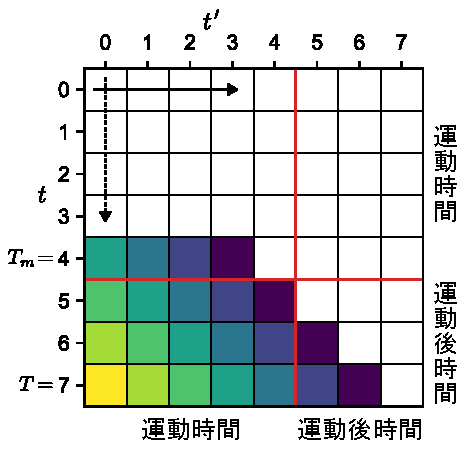
\includegraphics[width=0.35\textwidth]{./figures/minimum_variance.pdf}
  \caption{式 \ref{eq:mim_var_f} における和の順序交換の概念図 ($T=7$ とした場合).色付きのマスは時刻 $t, t'\quad (T_m \leq t \leq T, 0\ \leq t' \leq t-1)$ における $\left(\mathbf{A}^{t-t'-1} \mathbf{B}\right)\left(\mathbf{A}^{t-t'-1} \mathbf{B}\right)^{\top}$ の値を意味する.}
  \label{fig:minimum_variance}
\end{SCfigure}

ここで 
\begin{equation}
V_{t'}:=\sum_{t=\max(t'+1, T_m)}^{T} \left[\left(\mathbf{A}^{t-t'-1} \mathbf{B}\right)\left(\mathbf{A}^{t-t'-1} \mathbf{B}\right)^{\top} \right]_{1,1}
\end{equation}
とすると,$\mathbf{P}=\mathrm{diag}(V_0, \ldots, V_{T-1})\in \mathbf{R}^{T\times T}$および $\mathbf{q}=\mathbf{0} \in \mathbf{R}^{T}$と置くことで,$\mathcal{F}=\mathbf{u}^\top \mathbf{P}\mathbf{u}+\mathbf{q} ^{\top}\mathbf{u}$と書ける.この場合,第2項は0であるので,第1項の係数は結果に影響しない.

次に等式制約を求める.$\mathbb{E}\left[\mathbf{x}_{t}\right] = \mathbf{x}_f\quad (T_m\leq t \leq T)$を変形すると,
\begin{equation}
\sum_{t'=0}^{t-1} \mathbf{A}^{t-t'-1} \mathbf{B} u_{t'}=\mathbf{x}_f-\mathbf{A}^{t} \mathbf{x}_{0}
\end{equation}
となる.左辺について
\begin{equation}
\mathbf{C}_{(t-T_m)n+1:(t-T_m+1)n+1,\ t'}=
\begin{cases}
    \mathbf{A}^{t-t'-1} \mathbf{B} & (0\leq t'\leq t-1) \\
    \mathbf{0} & (t\leq t'\leq T-1)
\end{cases}\in \mathbb{R}^n 
\end{equation}
および,右辺について
\begin{equation}
\mathbf{d}_{(t-T_m)n+1:(t-T_m+1)n+1}=\mathbf{x}_f-\mathbf{A}^{t} \mathbf{x}_{0} \in \mathbb{R}^n 
\end{equation}
とすることで,等式制約が書き下せる.ただし,$[\cdot]_{i:j}$はベクトルあるいは行列の $i$番目から $j$番目までを取り出す操作を意味する.このように,$\mathbf{P}, \mathbf{q}, \mathbf{C}, \mathbf{d}$を設定すると,等式制約下の二次計画問題を用いて $\mathbf{u}$を求めることができる.

\printbibliography[segment=\therefsegment,heading=subbibliography,title={参考文献}]
\addcontentsline{toc}{section}{参考文献}
\end{document}